\chapter{Introduction}
\label{sec:introduction}

\section{Motivation}

Text Analysis sequence:

%
% text analysis sequence
%
\begin{center}
\begin{figure}[htbp]
\label{fig:text_analysis}
	\centering
	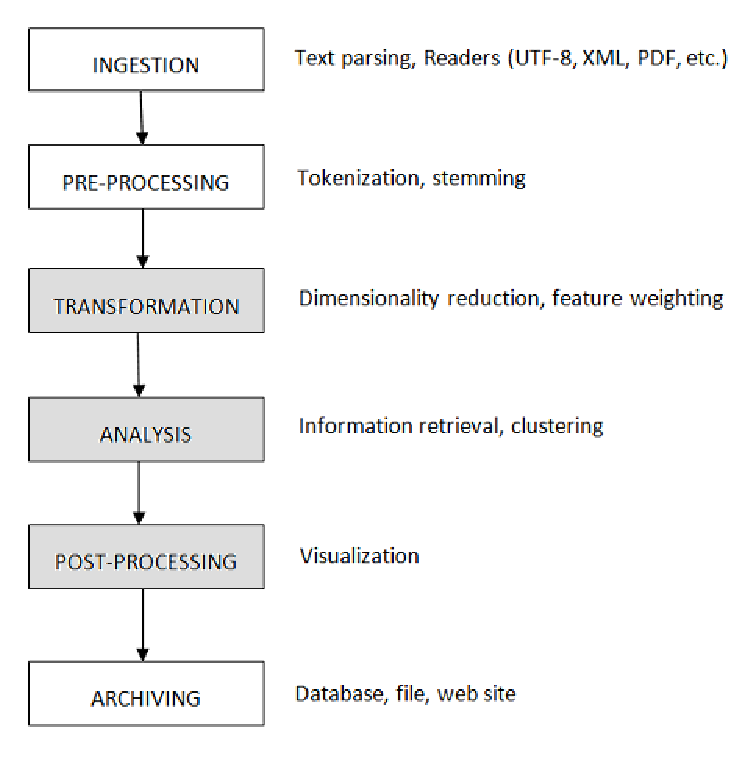
\includegraphics[width=\ScaleIfNeeded]{img/text_analysis} 
 % or [scale=0.5]
	\caption[Text analysis sequence]%
           {Text analysis sequence}
\end{figure}

This thesis contributes  for addressing the points presented above. The research focus is automatic identification of the main topics in a set of documents, returned as results to user queries. Research is done in analysis and visualization phases of the text analysis sequence diagram\ref{fig:text_analysis}.



\section{Goal and scope of work}
This works contributes with the following:
\begin{list}{}{}
\item Evaluation of the $ WCC $ algorithm, proposed for unsupervised topic labeling of clusters\cite{Stein04topicidentification}.
\item Proposition for improving $ WCC $ algorithm, using topic identification based on external knowledge. For this purpose, a light-weight ontology has been developed, in order to be used as a reference to external semantic knowledge. 
\item Software application for executing an IR process is developed. It presents a visualization of the main concepts contained in a document set in the form of a tag cloud.
\end{list}

\section{Outline}
This chapter motivates the presented research, and summarizes its contributions. It also offers a general overview to the problem of text analysis, common to most IR systems. \\
Chapter 2 gives the theoretical foundations for preprocessing and transformation phases of text analysis, and reviews a specific technique for information retrieval, called Latent Semantic Analysis. \\
Chapter 3 contains the contribution related to evaluation of $WCC$ algorithm, and a proposition for its improvement, by using a light-weight ontology developed for this purpose. It contains the analytical phase of text analysis problem. \\
Chapter 4 refers to the post-processing phase of text analysis, giving the visualization means to present the concepts retrieved from a document set. \\
The software contribution is given in Chapter 5. Finally in Chapter 6, this work concludes with evaluation of results and outlook.\\


We are now in the years before the Semantic Web, or Web 3.0. In the past years there has been major research in the fields of Information Retrieval, and improving search systems. Major companies like Google offer already products implementing techniques from the field of IR or semantics, in order to improve precision of search results, and increase user satisfaction.
However, despite the major research done in the field, the implementation of these techniques is still relatively limited on a business scale.\\

While many web-based search engines and applications implement techniques and tools from IR and semantic web, search functionality implemented in companies still relies mostly on full-text based search. \\


In order to create automatic modeling, processing, and analysis of unstructured text (LSA)\\

and labeling, and classification of unstructured text(Clustering and topic identification), we investigate the implementation of IR techniques for business needs in CoreMedia AG.\\

\section{Motivation}
Full-text search delivers a large number of results and does not handle synonymy and polysemy well. This problem can be partially solved by using IR technique to cope with polysemy and synonymy (such as LSA), and to use clustering for categorization of search results.\\
However, when using clustering, another issue arises - how to automatically identify category labels.\\

\section{Goal and scope of this work}
The goal of this work is to investigate implementation of IR technique LSA for handling ambiguous search in the use case of CoreMedia AG, Hamburg. In order to categorize search results, and provide better user experience, categorization of search results has been proposed, and a cluster labeling algorithm investigated. the implementation of IR and semantic technologies for business needs, in order to improve user experience with search systems.\\
Investigations have been made in three topics: use of ontologies to add semantic meaning to unstructured texts, use of IR techniques for document retrieval (LSA), and use of clustering technique and topic identification algorithm for categorizing search results.\\

\section{Thesis Structure}

Text analysis: methods for \\
searching - IR\\
labeling - TI algo\\
analyzing document collections - LSA, clustering\\

challenges:\\
- too much information to process manually (need automation)
data ambiguity\\

- ambiguous queries lead to information overload and topic confusion (IR)\\
- determine topics in text collections and identify most important relationships (Topic detection and association); clustering and visualization and key analysis methods\\

active text analysis research, implementation of techniques in business environment, for business needs? \\


----------------------------------\\
----------------------------------\\
Identifying the main concepts in texts is the subject of many research studies in the field of information retrieval and data mining. \\

This work investigates the implementation of Latent Semantic Analysis (LSA) for discovering the main concepts in texts, in order to present an overview of the text content in the form of a tag cloud.\\


During the last decade there have been constant optimizations in information retrieval effectiveness, making web search the preferred source of finding information. A substantial part of information retrieval deals with providing access to unstructured information in various domains. \gls{IR} refers to finding material (usually documents) of an unstructured nature (usually text) that satisfies an information need from within large collections (usually stored on computers) \cite{Mann08}. Many people today use methods from the field of IR when they use a search engine online, or search through their emails. In this context "unstructured data" refers to data which does not have a clear structure.\\

\gls{IR} technologies find wide application - in search engines, for browsing or filtering document collections, for further processing a set of retrieved documents. Before retrieval the documents are indexed, otherwise at each search, they would have to be scanned through for each query. The index maps the words or terms back to the documents where they occur. A method for document indexing, which is applied in this work, is called \gls{LSA}. It indexes the document collection by representing it as a reduced matrix of words and documents. \gls{LSA} representation improves \gls{IR} performance with respect to a basic problem of word-matching search - synonymy, or the case when more than one term describe the same concept. \\

While \gls{IR} deals with retrieval of documents, other systems manage content, such as documents. Content management includes a set of technologies and processes that support the creation, management and publication of content in any form or medium. Content may be documents, multi-media files, or any other file types that follow content lifecycle and require management. \gls{CMS} vary depending on their purpose and target environments - there are \gls{CMS} for the web, for enterprise, for mobile devices, as well as \gls{CMS} for managing collection of documents. \\

\section{Motivation and objective}
\label{sec:introduction:motandobj}  
A drawback of the classical \gls{LSA} implementation as an \gls{IR} method is the low precision of the returned results. A previous work by David Mugo \cite{mugo10} has investigated the improvement of \gls{LSA} precision performance by annotating the document collection and including the anotations used in \gls{LSA}. In his work, Mugo constructs a concept-document matrix from the annotations used, and concatenates it with the word-document matrix normally generated in \gls{LSA} process. The proposed solution, however, results in a slow speed of \gls{LSA}, and has left Mugo's hypothesis open. \\

Taking into consideration the results from Mugo's work, the current project has several objectives to reach. It will investigate the implementation of \gls{LSA} method for improving information retrieval in a domain-specific document management system with respect to context-based search. A further investigation will be made on improving the precision performance of \gls{LSA} method by using semantic annotations, and on finding an adequate way to present the results of \gls{LSA} as a tag cloud. And finally, it will be investigated how to use the tag cloud as a form of a relevance feedback to control \gls{LSA} method. \\

In the context of the stated objectives, semantic annotations are meta data annotations used to add information to unstructured data, or to the document collection. Semantic annotations are based on an ontology in our case, specifically developed for the domain of interest CoreMedia \gls{CMS}. Ontologies are used to capture some knowledge about a certain domain, by describing the concepts of the domain and the relationships between them. To further clarify the objectives, relevance feedback is an \gls{IR} technique, used to influence the retrieved results based on the user's preference. It allows the user to modify the initial tag cloud by selecting the most relevant words. The tag cloud is then re-generated from \gls{LSA} results with the relevance feedback posted as a query. \\

\section{Outline}
\label{sec:introduction:outline}
The reminder of this work is organized as follows. Chapter \ref{sec:docmanagsystem} describes in more detail what a document management system is, and provides an overview of the general structure of DocMachine 2.0, the \gls{CMS} deployed at CoreMedia AG. Chapter \ref{sec:semannot} presents the basic concepts of ontologies and document annotations based on ontologies. In Chapter \ref{sec:lsa} an overview of latent semantic analysis method is given, as well as an approach for improving \gls{LSA}'s precision by including semantic annotations in the method. Chapter \ref{sec:implementation} presents the prototype implementation and makes an evaluation of the results achieved in this work. And finally, conclusions are drawn in Chapter \ref{sec:conclusion}, along with some limitations of the current study and outlook for a future research.   \\ 
